\documentclass[a4paper]{article}

\usepackage[utf8]{inputenc}
\usepackage[T1]{fontenc}
\usepackage{textcomp}
\usepackage{multicol}
\usepackage{verbatim,listings,minted}
\usepackage{mathtools,amssymb,amsthm}
\usepackage[a4paper, total={6in, 8in}]{geometry}
\usepackage[francais]{babel}

%============header and foot============
\usepackage{fancyhdr}
\pagestyle{fancy}
\renewcommand\headrulewidth{1pt}
\fancyhead[L]{\bfseries TP5 MDE}
% \fancyhead[R]{\includegraphics[scale=0.05]{image.png}}
\fancyfoot[L]{CHASSAGNOL Rémi}
\fancyfoot[R]{2023-2024}

%================image=================
\usepackage{graphicx}

%------------------------------------------------------------------------------%
%                                   document                                   %
%------------------------------------------------------------------------------%

\begin{document}
\begin{titlepage}
\begin{center}

    \textsc{\LARGE TP IDM}\\[0.5cm]

    {\huge \bfseries Génération de flux parallèles de nombres pseudo-aléatoires\\[3cm]}

      \centering
      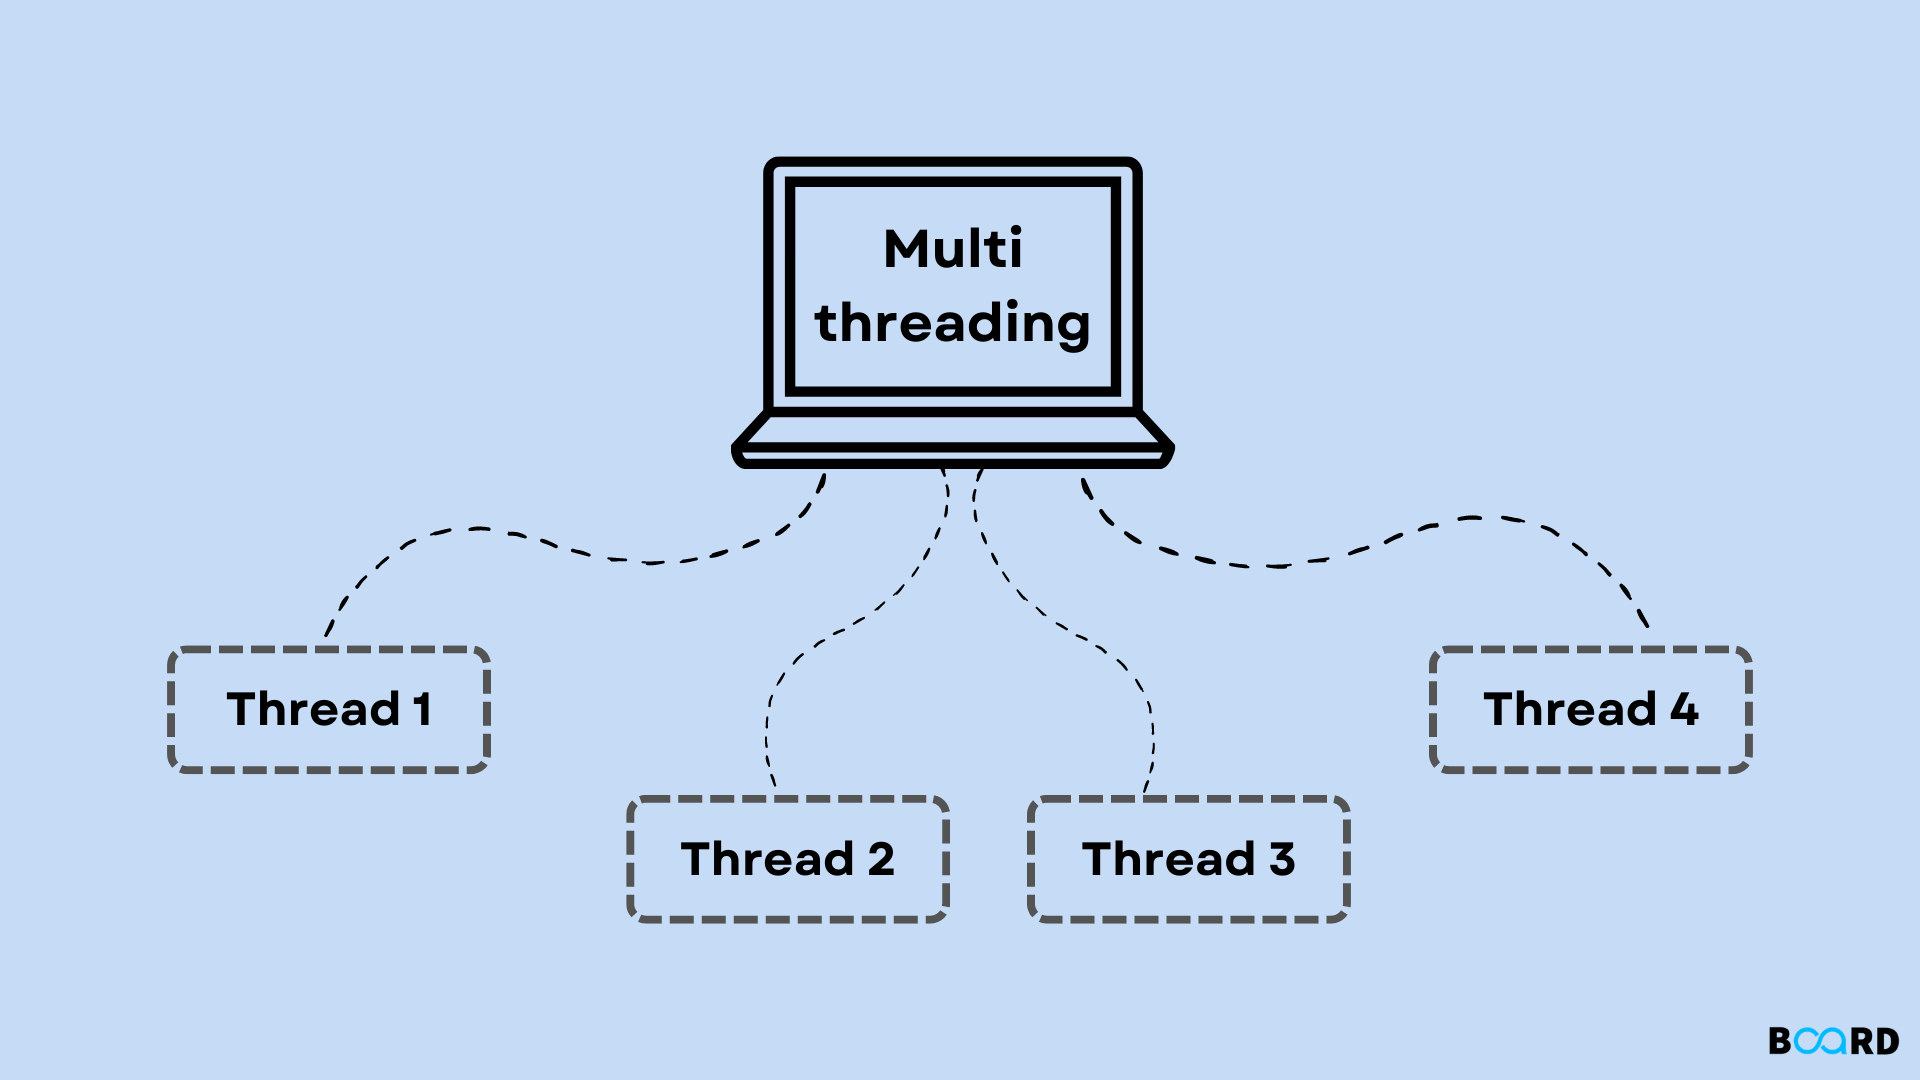
\includegraphics[scale=0.3]{./img/banner.png}

      \vspace*{\fill}

    \begin{multicols}{2}
      \large
      CHASSAGNOL Rémi\\

      \columnbreak

      \large
      \emph{Professeur:} HILL David\\
    \end{multicols}

    \textsc{\today}

  \end{center}
\end{titlepage}

\clearpage
\tableofcontents
\clearpage

\section{Introduction}

L'objectif de ce TP est d'utiliser le un générateur de nombres pseudo-aléatoires
pour réaliser des calculs en parallèle. Pour générer les nombres nous
utiliserons l'implémentation de Mersenne Twister fournie par la bibliothèque
CLHEP. Nous commencerons par détailler l'installation de la bibliothèque, puis
nous testerons la répétabilité des séquences de nombres générés aléatoirement.
Ensuite, nous traiterons l'exemple simple du calcul du nombre $\pi$, d'abord en
séquentiel, puis en parallèle. Avant de conclure, nous traiterons un exemple
plus complexe sur la génération de mots et de bases nucléiques.

\clearpage

\section{Utilisation de CLHEP}

Dans cette première section nous allons voir comment installer la bibliothèque
CLHEP. Pour simplifier la gestion des dépendances, ce projet utilise des
sous-modules git.

Le clonage des sous-modules ne se fait pas automatiquement lors du clonage du
projet. Pour avoir accès aux sous-modules, il faut utiliser les commandes
du listing \ref{git-sm}.

\begin{listing}[ht!]
\begin{minted}{bash}
  git submodule init
  git submodule update
\end{minted}
\caption{Synchronisation des sous-modules git.}
\label{git-sm}
\end{listing}

L'utilisation des sous-modules évite surcharger les serveurs contenant les
dépôts en stockant plusieurs fois le même code. De plus, ils permettent de
facilement cloner les dépendances (cela est plus simple que de télécharger la
bibliothèque manuellement).\\

Pour compiler la bibliothèque, il faut utiliser le script \lstinline{build.sh}
du répertoire \lstinline{lib}. Ce script va permettre de compiler et d'installer
la bibliothèque (fichiers d'entêtes, bibliothèque statiques, \dots) dans le
répertoire \lstinline{lib/CLHEP-lib}. Ensuite, on peut compiler le projet en
utilisant CMake.

\section{Test du générateur}

Avant de commencer les calculs, assurons-nous que le générateur produit bien
toujours les même séquences de nombres lorsqu'il charge les fichiers de
statuts.\\

La générations des fichier de statuts se fait avec la méthode
\lstinline{saveStatus} et le chargement des fichiers se fait avec la méthode
\lstinline{restoreStatus}. Dans la fonction \lstinline{question2}, nous générons
dans un premier temps des fichiers de statuts, et chaque statuts est séparé par
un certain nombre de tirage de nombre pseudo-aléatoires. Les tirages sont
sauvegardés dans un tableau.

Dans un second temps, nous restaurons les statuts et nous vérifions que les
tirages sont les même que ceux sauvegardés précédemment. Ici, nous utilisons un
\lstinline{assert} pour tester l'égalité des nombres. Si les nouveaux nombres
générés ne sont pas égaux à ceux sauvegardés, le programme s'arrête avec un code
erreur. Si le programme se termine sans échouer, le test du générateur est
valide.\\

À noter que ce test basique ne permet pas de valider avec certitude le bon
fonctionnement du générateur. Nous nous contenterons cependant de ce test étant
donné le fait la répétabilité de Mercenne Twister peut être prouvée
mathématiquement. Ici, nous vérifions juste que l'implémentation fonctionne sur
un petit nombre de tirages.

\section{Calcul de pi}

Maintenant que nous avons vérifier le bon fonctionnement du générateur, nous
allons réaliser un simple calcul de $\pi$ en utilisant la méthode de Monte
Carlo. Le calcul sera fait de façon séquentielle dans un premier temps, puis de
façon parallèle dans un second temps.

\subsection{Génération des fichiers de statuts}

Pour pouvoir paralléliser les calculs, il faut préalablement générer des
fichiers de statuts pour pouvoir lancer le générateur à partir d'un point donné.
Sans cette étape, les calculs lancés en parallèles utiliseront la même séquence
de nombre pseudo-aléatoires, ce qui rendra la parallélisation inutile.\\

La génération des fichiers de statuts se fait à l'aide de la fonction
\lstinline{question3}. On peut configurer le nombre de fichiers à générer ainsi
que le nombre de tirages séparant chaque statuts. Pour la suite, on utilisera
les valeurs par défauts des paramètres. Il est important d'utiliser cette
fonction avant de tester les autres fonctionnalité du programme car les fichiers
de statuts seront utilisés dans les autres questions. Les fichiers générés sont
nommés mt3\_1, mt3\_2, \dots

\subsection{Calcul séquentiel}

Dans un premier temps, nous allons réaliser le calcul de $\pi$ de façon
séquentielle. Cela va permettre de vérifier notre algorithme et simplifiera la
parallélisation.\\

Pour le calcul séquentiel, nous utilisons la fonction \lstinline{question4} qui
réalise plusieurs calculs de $\pi$ et qui calcule la moyenne des résultats pour
avoir un valeur approchée. Cette fonction prend en paramètre le nombre de
réplications du calcul ainsi que le nombre de tirages pour chaque réplication.
Pour chaque réplication, on restaure un statut du générateur puis on utilise la
fonction \lstinline{computePi}. Ici, il n'est pas vraiment nécessaire de
restaurer les statuts du générateur à chaque itération, cependant, cela permet
de facilement tester le code qui sera parallélisé par la suite. Le code de la
fonction est visible sur le listing \ref{fn-qf}.

\begin{listing}[ht!]
\begin{minted}{CPP}
void question4(size_t nbReplications, size_t nbDraws,
               const std::string &fileName) {
    CLHEP::MTwistEngine mt;
    double sumPI = 0;

    timerStart();
    for (size_t i = 0; i < nbReplications; ++i) {
        mt.restoreStatus(cat(fileName, i).c_str());
        sumPI += computePi(mt, nbDraws);
    }
    timerEnd();

    std::cout << std::setprecision(10) << "pi: " << sumPI / nbReplications
              << "; time: " << timerCountMs() << std::endl;
}
\end{minted}
\caption{Fonction question4.}
\label{fn-qf}
\end{listing}

La fonction permet aussi de mesurer le temps de calcul en utilisant les macros
visibles sur le listing \ref{macro-timer}. Ces macro permette d'avoir une
approximation du nombre de mili-secondes écoulées durant un calcul. Ici, on
choisit une précision à la micor-seconde ce qui est très élevé étant donnée le
fait que l'exécution des calculs peut prendre plusieurs secondes. Cependant,
cela reste intéressant s'il on souhaite faire des mesure plus précises.

\begin{listing}[ht!]
\begin{minted}{CPP}
#define timerStart() auto _start = std::chrono::high_resolution_clock::now();
#define timerEnd() auto _end = std::chrono::high_resolution_clock::now();
#define timerCountMs()                                                         \
    std::chrono::duration_cast<std::chrono::microseconds>(_end - _start)       \
            .count() /                                                         \
        1000.0
\end{minted}
\caption{Macro timer.}
\label{macro-timer}
\end{listing}

Ici, le calcul prend plus d'une minute pour s'exécuter. Dans la partie suivante,
nous allons comparer ce temps de calcul avec celui obtenu en parallélisant les
calculs.

\subsection{Calcul parallèle}

Dans cette section nous allons paralléliser le calcul de $\pi$ avec la méthode
de Monte Carlo. Nous commencerons par utiliser un script bash qui crée des
processus, puis nous utiliserons les threads de la bibliothèque standard de C++.

\subsubsection{Utilisation d'un script}
\label{sec:script}

Ici, nous allons utiliser un script bash pour paralléliser les calculs.
L'objectif est de faire en sorte de pouvoir passer en argument du programme le
nom d'un fichier de statut à charger de sorte à pouvoir lancer plusieurs fois le
même programme en tâche de fond avec un fichier différent.\\

La fonction \lstinline{question5} est une version simplifiée de la fonction
\lstinline{question4} qui ne lance qu'une fois le calcul. La fonction prend
aussi en argument le nom du fichier de statut à charger pour initialiser le
générateur.

Le script utilisé pour lancer les processus est visible sur le listing
\ref{script}. Ici, on commence par vérifier que le projet est bien compilé et
que les fichiers de statuts ont bien été généré (dans le cas contraire, on fait
le nécessaire) avec la fonction \lstinline{checkSetup}. Ensuite on défini le nom
des fichiers de sortie du programme (le nom est configurable avec les argument
du script), puis on lance 10 processus en tâche de fond (utilisation du
\lstinline{\&} en fin de ligne) avec une boucle \lstinline{for}. Une fois
l'exécution terminée, les résultats sont stockés dans les fichiers du répertoire
\lstinline{out/}.

\begin{listing}[ht!]
\begin{minted}{bash}
#!/usr/bin/env bash

set -euo pipefail

checkSetup() {
  # ...
}

checkSetup

# configure output file
outputFile=pi
if [ $# -eq 1 ]; then
    outputFile=$1
fi
mkdir -p out

# compute pi
echo "computing pi"
for i in {0..9}; do
    echo "./build/tp5 ./build/mt3_$i"
    ./build/tp5 "./build/mt3_$i" > "./out/$outputFile$i.out" &
done

# wait and quit
time wait
echo "done"
\end{minted}
\caption{Script compute\_pi.sh}
\label{script}
\end{listing}

À noter qu'à la fin du script on utilise la commande \lstinline{wait} qui va
permettre d'attendre que tous les processus lancés en tâche de fond se terminent
pour quitter le programme. On emploie aussi la commande \lstinline{time} pour
mesurer le temps de calcul total (on considère que le temps de lancement des
processus est négligeable, on ne le prend donc pas en compte ici).\\

\begin{figure}[ht!]
  \centering
  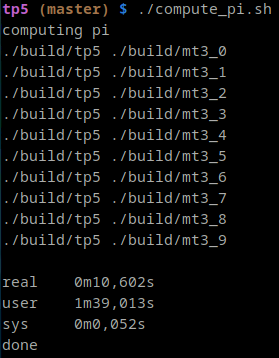
\includegraphics[scale=0.5]{./img/pi_script.png}
  \caption{Résultat du script lancé sur Ada.}
  \label{fig:script}
\end{figure}

Comme on peut le voir sur la figure \ref{fig:script}, le calcul prend environ
dix secondes ce qui est bien plus rapide que le temps de calcul séquentiel.

\subsubsection{Utilisation des threads}

La seconde solution utilise les threads de la bibliothèque standard de C++. Ici,
on utilise la fonction \lstinline{question6a} disponible en deux version, une
utilisant directement les threads, et une autre utilisant l'abstraction
\lstinline{std::future}. Les deux version utilisent la fonction
\lstinline{question5} présentée dans la section \ref{sec:script}.

\begin{listing}[ht!]
\begin{minted}{CPP}
void question6aFuture(const std::string &fileName, size_t nbDraw) {
    CLHEP::MTwistEngine mt;
    size_t i;

    timerStart();
    /* threads scope */ {
        std::future<void> pis[NB_REPLICATION];
        for (i = 0; i < NB_REPLICATION; ++i) {
            pis[i] = std::async(std::launch::async, question5, cat(fileName, i),
                                nbDraw);
        }
    }
    timerEnd();
    std::cout << "total time: " << timerCountMs() / 1000.0 << "s" << std::endl;
}
\end{minted}
\caption{Fonction question6aFuture.}
\label{fn-q6}
\end{listing}

\begin{figure}[ht!]
  \centering
  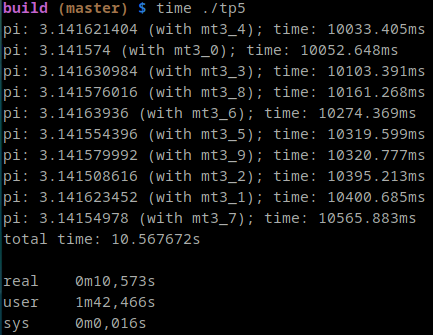
\includegraphics[scale=0.5]{./img/pi_threads.png}
  \caption{Résultat du script lancé sur Ada.}
  \label{fig:threads}
\end{figure}

Comme on peut le voir sur la figure \ref{fig:threads}, le temps de calcul est
similaire à celui du script ce qui est logique étant donné le fait que le même
nombre de thread a été utilisé.

\section{Gattaca}

\section{Génération de bases nucléiques}

\section{Conclusion}

\end{document}
